% =====================================================================
% CHƯƠNG 1: BỐI CẢNH AN TOÀN MẠNG VÀ MÔ HÌNH DỊCH CHUYỂN ZERO TRUST
% =====================================================================
\chapter{BỐI CẢNH AN TOÀN MẠNG VÀ MÔ HÌNH DỊCH CHUYỂN ZERO TRUST}
\label{chap:1}

% ---------------------------------------------------------------------
% 1.1. SỰ TIẾN HÓA CỦA HẠ TẦNG MẠNG DOANH NGHIỆP HIỆN ĐẠI
% ---------------------------------------------------------------------
\section{Sự tiến hóa của hạ tầng mạng doanh nghiệp hiện đại}
\label{sec:1_1}

Hạ tầng Công nghệ thông tin (CNTT) của các doanh nghiệp hiện đại đang trở nên ngày càng phức tạp và phân tán. Một tổ chức ngày nay có thể đồng thời vận hành nhiều mạng nội bộ, các văn phòng chi nhánh từ xa với hạ tầng riêng biệt, kết hợp với lực lượng lao động làm việc linh hoạt từ xa và hệ thống dịch vụ đám mây đa dạng.

Chính sự phức tạp này tạo ra những thách thức lớn đối với khả năng kiểm soát của các phương pháp bảo mật mạng dựa trên vành đai truyền thống (\textit{Perimeter-based Security}), bởi doanh nghiệp không còn sở hữu một ranh giới mạng vật lý duy nhất dễ dàng xác định. Hơn thế nữa, mô hình phòng thủ vành đai bộc lộ những hạn chế đáng kể: nếu kẻ tấn công vượt qua được bức tường lửa cửa ngõ, chúng có thể tiến hành di chuyển sang ngang (\textit{Lateral Movement}) trong hệ thống mạng nội bộ mà ít gặp phải rào cản hay cơ chế phát hiện chuyên sâu.

Bối cảnh này đã thúc đẩy sự phát triển của một tư duy an ninh mạng thế hệ mới mang tên Zero Trust (ZT - Không tin tưởng ngầm định).

\subsection{Sự bùng nổ của Điện toán đám mây và dịch vụ SaaS}
\label{subsec:1_1_1}

Trong quá trình tiến hóa hạ tầng, sự bùng nổ của Điện toán đám mây và các dịch vụ Phần mềm như một Dịch vụ (\textit{SaaS - Software as a Service}) đóng vai trò là tác nhân chuyển dịch cốt lõi thông qua 4 khía cạnh:

\begin{enumerate}
    \item \textbf{Sự dịch chuyển sang hạ tầng Đa đám mây (\textit{Multi-Cloud Migration}):} Doanh nghiệp chủ động chuyển dịch các tải công việc (\textit{workloads}) từ trung tâm dữ liệu nội bộ (\textit{On-premises Data Center}) sang vận hành trên các nền tảng điện toán đám mây công cộng như Amazon Web Services (AWS), Microsoft Azure, và Google Cloud Platform (GCP). Việc áp dụng các mô hình Hạ tầng dưới dạng Dịch vụ (\textit{IaaS - Infrastructure as a Service}) và Nền tảng dưới dạng Dịch vụ (\textit{PaaS - Platform as a Service}) khiến dữ liệu nghiệp vụ không còn nằm trong phạm vi bảo vệ vật lý thuộc quyền kiểm soát trực tiếp của doanh nghiệp.
    
    \item \textbf{Sự phổ cập của các ứng dụng SaaS nghiệp vụ:} Các công cụ làm việc cốt lõi của tổ chức như Microsoft 365, Google Workspace, Salesforce hay Zoom được triển khai rộng rãi theo mô hình SaaS. Cán bộ nhân viên truy cập trực tiếp vào các ứng dụng này qua trình duyệt web trên nền tảng Internet công cộng, giảm dần sự phụ thuộc vào việc kết nối tập trung về máy chủ ứng dụng nội bộ qua mạng LAN truyền thống.
    
    \item \textbf{Thay đổi bản chất luồng lưu lượng mạng (\textit{Network Traffic}):} Tuyến truyền tải dữ liệu truyền thống theo mô hình tập trung ($\text{Người dùng} \rightarrow \text{Mạng nội bộ} \rightarrow \text{Trung tâm dữ liệu}$) dần được thay thế bởi mô hình kết nối phân tán ($\text{Người dùng} \rightarrow \text{Internet công cộng} \rightarrow \text{Dịch vụ Đám mây/SaaS}$).
    
    \item \textbf{Hiện tượng giảm hiệu lực ranh giới bảo mật (\textit{De-perimeterization}):} Do lưu lượng dữ liệu từ người dùng đến ứng dụng Đám mây/SaaS nhiều trường hợp đi thẳng qua Internet thay vì qua cổng kết nối gateway của trung tâm dữ liệu nội bộ, các cơ chế kiểm soát đặt tại chu vi trung tâm có thể mất khả năng quan sát trực tiếp một phần lưu lượng truy cập này, từ đó làm giảm hiệu quả giám sát của các thiết bị truyền thống như Tường lửa (\textit{Firewall}) hay Hệ thống phát hiện và ngăn ngừa xâm nhập (\textit{IDS/IPS}).
\end{enumerate}

Tóm lại, sự kết hợp giữa hạ tầng Đa đám mây và các dịch vụ SaaS đã làm mờ ranh giới bảo mật vật lý duy nhất của doanh nghiệp, đặt ra yêu cầu chuyển dịch sang mô hình an toàn thông tin phù hợp hơn — Kiến trúc Bảo mật Zero Trust.

% ---------------------------------------------------------------------
% 1.2. PHÂN TÍCH LỖ HỔNG CỦA MÔ HÌNH BẢO MẬT CHU VI
% ---------------------------------------------------------------------
\section{Phân tích lỗ hổng của Mô hình bảo mật chu vi (Perimeter Security)}
\label{sec:1_2}

\subsection{Nguyên lý ``Castle-and-Moat'' và khái niệm vùng tin tưởng nội bộ}
\label{subsec:1_2_1}

Mô hình phòng thủ mạng truyền thống vận hành dựa trên tư duy quân sự cổ điển mang tên ``Lâu đài và Hào nước'' (\textit{Castle-and-Moat}). Trong mô hình này, tòa thành đại diện cho toàn bộ tài nguyên nội bộ của doanh nghiệp, còn bức tường thành và hào nước chính là ranh giới chu vi mạng đóng vai trò ngăn cách giữa môi trường bên trong và bên ngoài.

\begin{figure}[htbp]{Kiến trúc bảo mật mạng truyền thống dựa trên phân vùng tin tưởng (Traditional Network Security Architecture).}
    \centering
    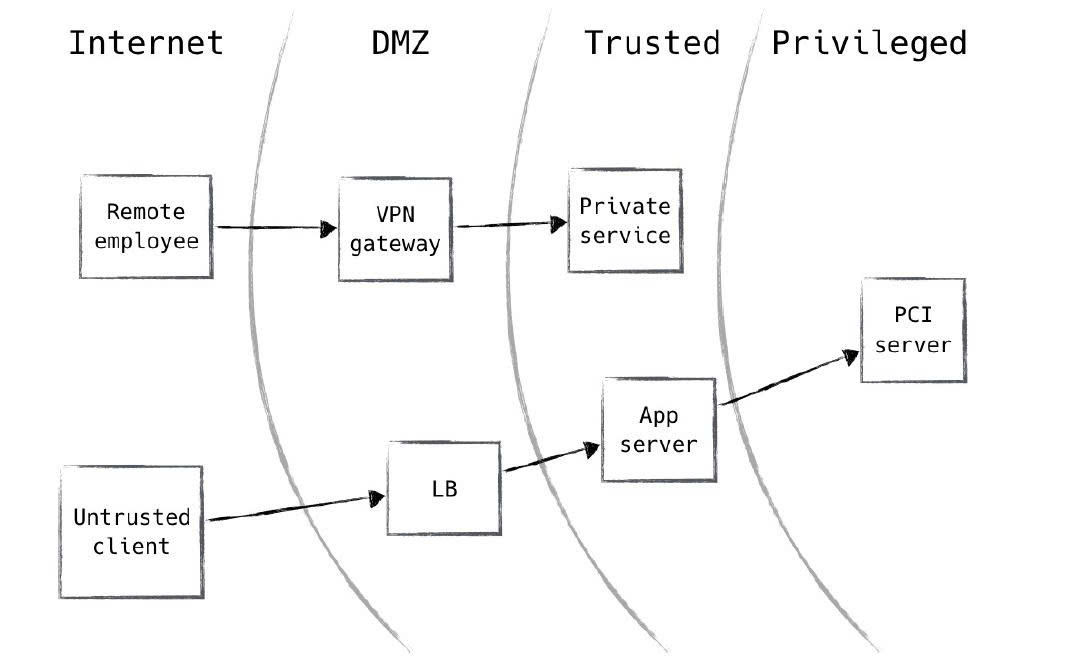
\includegraphics[width=0.85\textwidth]{1.jpg}
    \label{fig:1_1}
\end{figure}

Như được minh họa trong Hình~\ref{fig:1_1}, kiến trúc truyền thống phân chia mạng thành các vùng (\textit{zones}) chứa cấp độ tin cậy (\textit{Level of Trust}) tăng dần từ trái sang phải:
\begin{itemize}
    \item \textbf{Mạng không tin tưởng (\textit{Internet / Untrusted Zone}):} Nơi chứa các đối tượng bên ngoài như nhân viên làm việc từ xa (\textit{Remote employee}) hoặc khách hàng chưa được xác minh (\textit{Untrusted client}).
    \item \textbf{Vùng đệm cách ly (\textit{DMZ - Demilitarized Zone}):} Nơi đặt các thiết bị giao tiếp cửa ngõ như cổng kết nối VPN (\textit{VPN gateway}) và bộ cân bằng tải (\textit{Load Balancer - LB}) nhằm tiếp nhận luồng dữ liệu từ bên ngoài.
    \item \textbf{Vùng tin tưởng nội bộ (\textit{Trusted Zone}):} Nơi chứa các dịch vụ nội bộ (\textit{Private service}) và máy chủ ứng dụng (\textit{App server}).
    \item \textbf{Vùng đặc quyền / Bảo mật cao (\textit{Privileged Zone}):} Nơi lưu trữ tài sản nhạy cảm như máy chủ cơ sở dữ liệu thanh toán (\textit{PCI server}), thường chỉ cho phép truy cập trực tiếp từ máy chủ ứng dụng.
\end{itemize}

Bản chất cốt lõi của mô hình này nằm ở triết lý: ``Niềm tin xác định mức độ bảo mật tối thiểu bắt buộc'' (\textit{Trust defines the minimum required security}). Khi một thiết bị nằm bên trong ``Vùng tin tưởng nội bộ'', nó thường mặc định được coi là an toàn, dẫn đến việc hệ thống giảm bớt các cơ chế kiểm tra chuyên sâu, nhiều luồng dữ liệu nội bộ không được mã hóa mặc định và hạn chế việc xác thực lại liên tục giữa các nút mạng ngang hàng.

\begin{figure}[htbp]{Sự tích tụ ngoại lệ tường lửa khi kết nối mạng văn phòng (Corp), vùng đệm (DMZ) và mạng đối tác (Partner).}
    \centering
    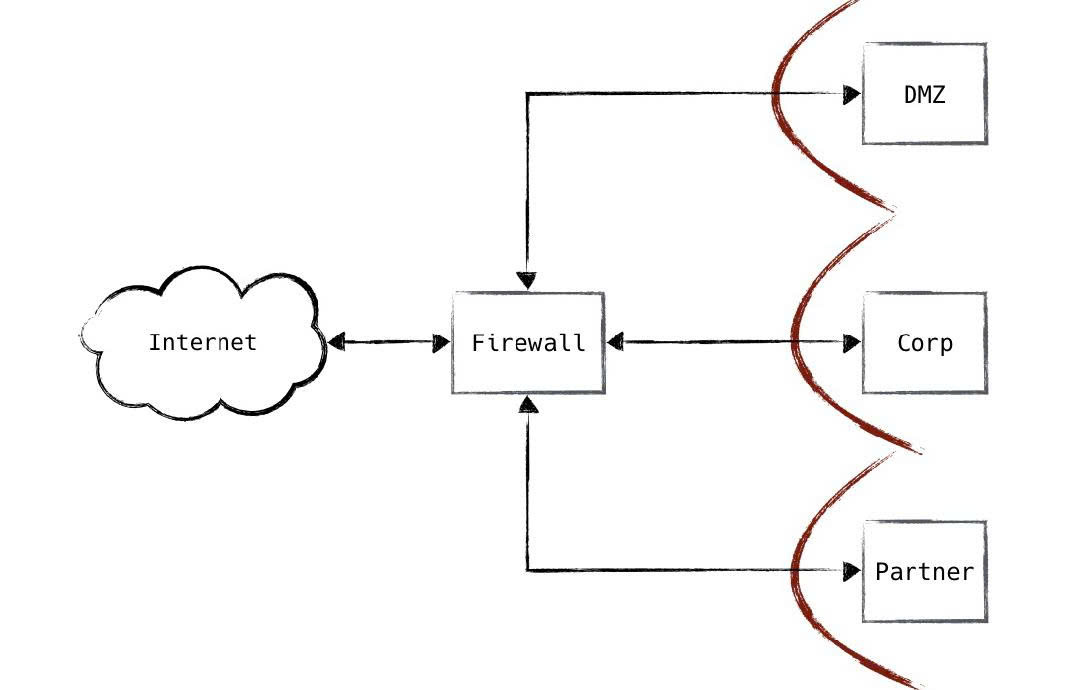
\includegraphics[width=0.75\textwidth]{2.jpg}
    \label{fig:1_2}
\end{figure}

Tuy nhiên, khi doanh nghiệp mở rộng kết nối với các bên thứ ba và mạng đối tác (\textit{Partner Network}), bức tường lửa chu vi bắt buộc phải tạo các quy tắc ngoại lệ (\textit{Rule Holes}) như trong Hình~\ref{fig:1_2}. Sự tích tụ theo thời gian của các quy tắc ngoại lệ này làm suy yếu ranh giới bảo mật cứng ban đầu.

\begin{figure}[htbp]{Sự tương tác kết nối chéo giữa Mạng văn phòng doanh nghiệp (Corp) và Trung tâm dữ liệu sản xuất (DC/Production).}
    \centering
    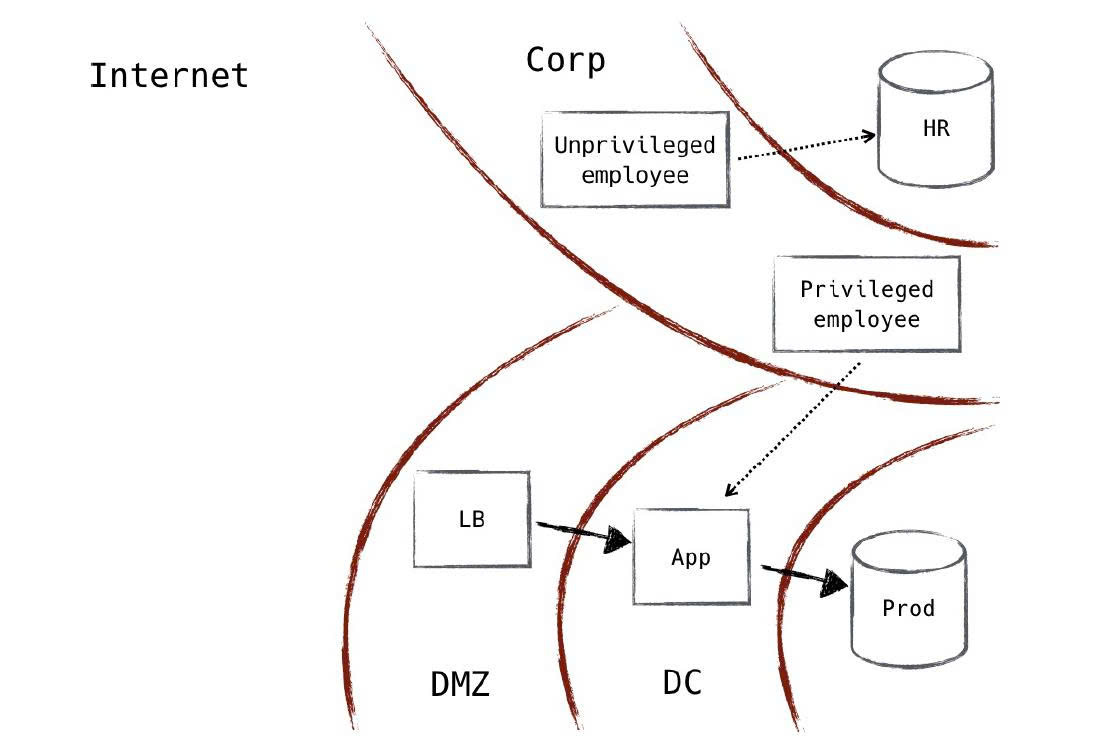
\includegraphics[width=0.80\textwidth]{4.jpg}
    \label{fig:1_3}
\end{figure}

Hình~\ref{fig:1_3} minh họa thực tế tương tác phức tạp giữa mạng doanh nghiệp (\textit{Corp}) và trung tâm dữ liệu sản xuất (\textit{DC}): nhân viên không có đặc quyền (\textit{Unprivileged employee}) phải truy cập CSDL Nhân sự (\textit{HR}), trong khi nhân viên đặc quyền (\textit{Privileged employee}) kết nối trực tiếp vào máy chủ ứng dụng (\textit{App}) tại trung tâm dữ liệu. Các luồng kết nối chéo này có thể biến phân vùng bảo mật thành điểm nhảy (\textit{pivoting points}) cho kẻ tấn công nếu một thiết bị bị chiếm quyền kiểm soát.

\subsection{Hạn chế của Tường lửa chu vi và kỹ thuật khai thác kết nối Outbound}
\label{subsec:1_2_2}

Sự chuyển dịch sang bộ giao thức TCP/IP mang lại sự linh hoạt nhưng đòi hỏi cơ chế kiểm soát chặt chẽ. Mặc dù giao thức TCP/IP hỗ trợ kết nối hai chiều (\textit{Bi-directional communication}), nhiều cấu hình tường lửa chu vi truyền thống vì lý do tối ưu vận hành thường áp dụng chính sách nới lỏng kiểm soát đối với luồng lưu lượng đi ra (\textit{Outbound Traffic}) so với luồng đi vào (\textit{Inbound Traffic}).

\begin{figure}[htbp]{Tiến trình tấn công do máy nạn nhân khởi tạo kết nối đi ra (Outbound) vượt qua tường lửa chu vi.}
    \centering
    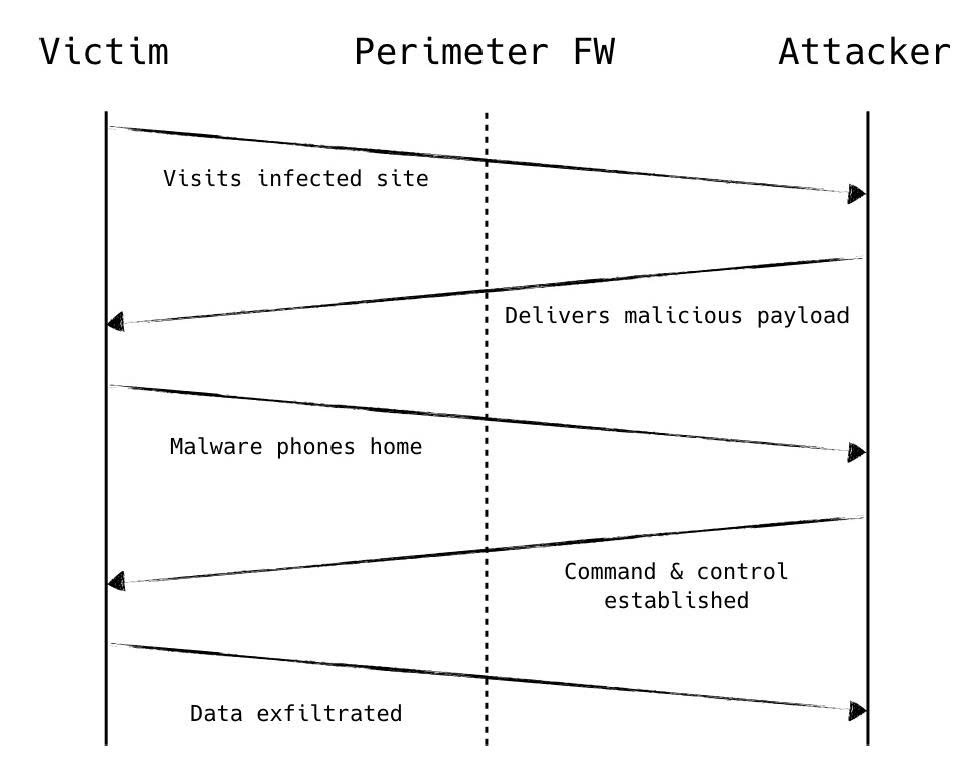
\includegraphics[width=0.75\textwidth]{3.jpg}
    \label{fig:1_4}
\end{figure}

Sơ đồ trình tự trong Hình~\ref{fig:1_4} mô tả chi tiết cách kẻ tấn công lợi dụng chính sách luồng Outbound nới lỏng để xâm nhập qua tường lửa chu vi (\textit{Perimeter FW}) thông qua một chuỗi kết nối do chính thiết bị nạn nhân (\textit{Victim}) khởi tạo:
\begin{enumerate}
    \item \textbf{Khởi tạo kết nối (\textit{Visits infected site}):} Nạn nhân truy cập vào trang web bị lây nhiễm hoặc mở tệp đính kèm chứa mã độc từ email lừa đảo (\textit{Phishing}).
    \item \textbf{Tải mã độc (\textit{Delivers malicious payload}):} Máy chủ của kẻ tấn công (\textit{Attacker}) gửi gói dữ liệu độc hại về máy nạn nhân.
    \item \textbf{Mã độc gọi về C2 (\textit{Malware phones home}):} Mã độc thực thi trên máy nạn nhân, chủ động khởi tạo một kết nối TCP đi ra (\textit{Outbound}) gửi về máy chủ điều khiển C2 (\textit{Command and Control}). Do tường lửa cửa ngõ thường cho phép lưu lượng web Outbound thông thường đi qua, kết nối này dễ dàng được thiết lập.
    \item \textbf{Thiết lập Command \& Control (\textit{C2 Established}):} Kênh điều khiển hai chiều được thiết lập hoàn tất dưới dạng đường hầm ngược (\textit{Reverse Shell}), cho phép kẻ tấn công gửi lệnh điều khiển vào bên trong mạng nội bộ.
    \item \textbf{Rút hái dữ liệu (\textit{Data exfiltrated}):} Dữ liệu nhạy cảm thu thập được bị đóng gói và gửi ngược ra ngoài Internet thông qua chính kênh kết nối Outbound đã khởi tạo.
\end{enumerate}

\subsection{Sơ đồ tiến trình tấn công điển hình và nguy cơ di chuyển sang ngang}
\label{subsec:1_2_3}

Một khi kẻ tấn công đã tạo được kênh giao tiếp ngược vào bên trong mạng doanh nghiệp, chúng bắt đầu tận dụng sự thiếu vắng các rào cản kiểm soát nội bộ để tiến hành mở rộng phạm vi ảnh hưởng qua các kỹ thuật cốt lõi:
\begin{itemize}
    \item \textbf{Trích xuất thông tin xác thực (\textit{Credential Theft}):} Thu thập trái phép tài khoản, mật khẩu, token xác thực hoặc khóa mã hóa.
    \item \textbf{Leo thang đặc quyền (\textit{Privilege Escalation}):} Khai thác lỗ hổng hoặc dùng credential chiếm đoạt để nâng đặc quyền lên quyền quản trị (\textit{Admin/Root}).
    \item \textbf{Di chuyển sang ngang (\textit{Lateral Movement}):} Sử dụng quyền hạn và thông tin xác thực đã chiếm đoạt để dò quét, kết nối và truy cập sang các máy trạm và máy chủ khác trong mạng nội bộ.
\end{itemize}

\begin{figure}[htbp]{Sơ đồ tiến trình tấn công 10 bước xâm nhập mạng doanh nghiệp và đánh cắp dữ liệu sản xuất (Example Attack Progression).}
    \centering
    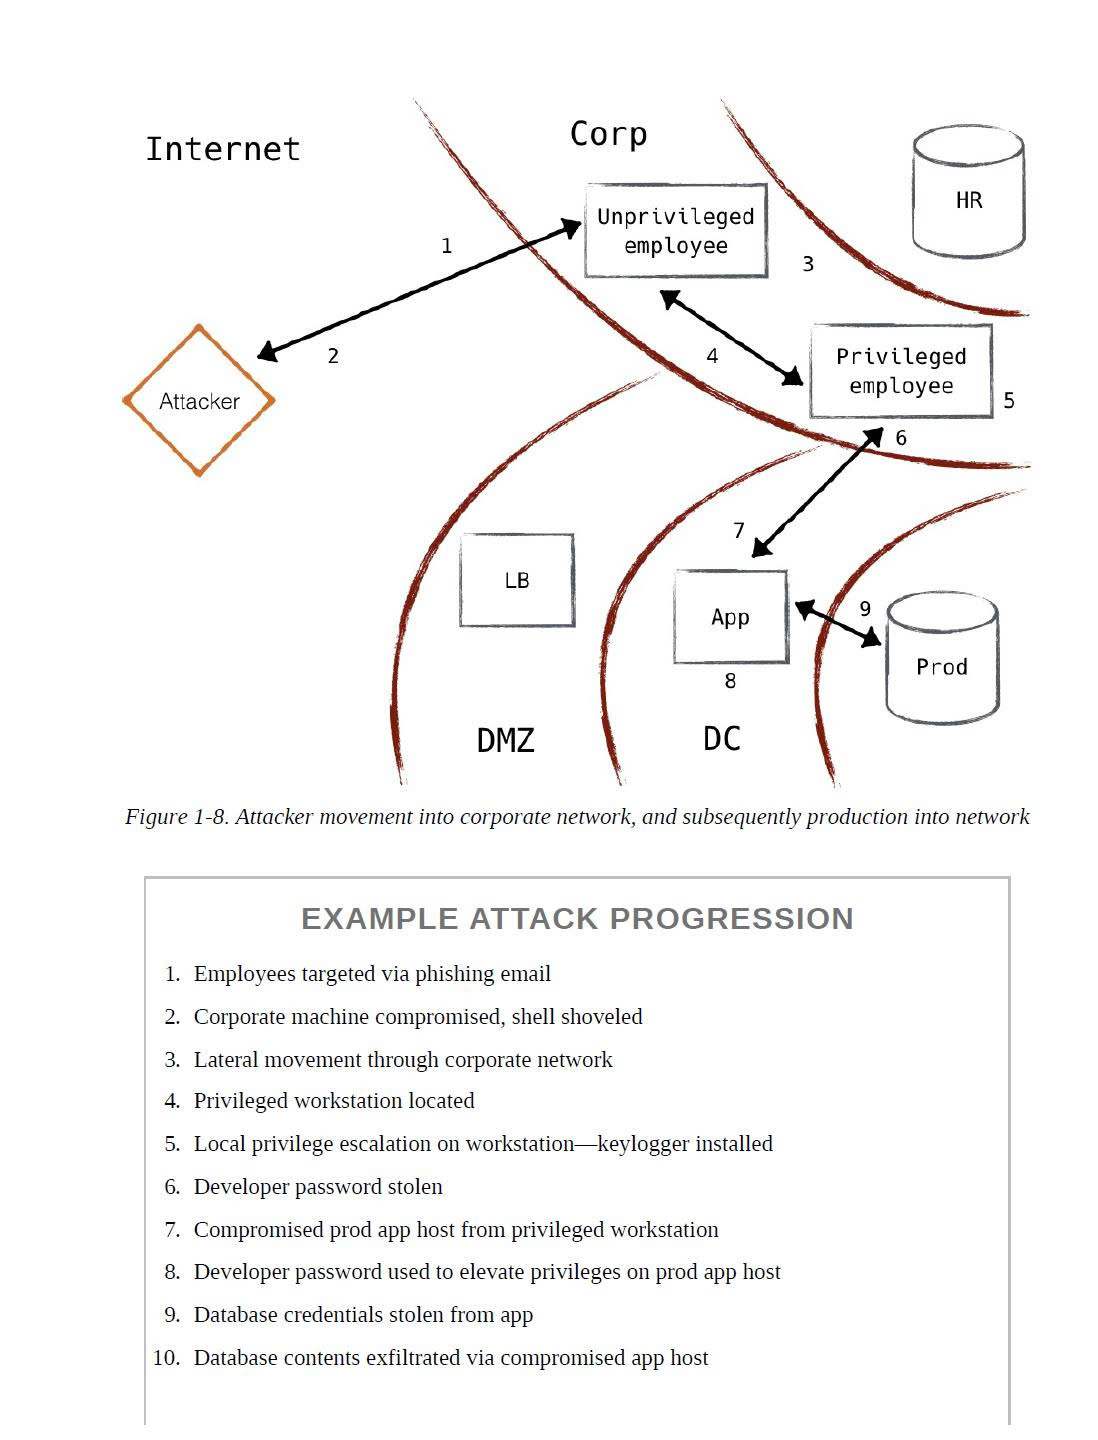
\includegraphics[width=0.82\textwidth]{5.jpg}
    \label{fig:1_5}
\end{figure}

Hình~\ref{fig:1_5} phác thảo kịch bản tấn công thực tế gồm 10 giai đoạn thể hiện chuỗi liên kết của các kỹ thuật trên:
\begin{enumerate}
    \item[\textbf{a)}] \textbf{Tấn công Phishing:} Kẻ tấn công nhắm mục tiêu vào nhân viên qua email lừa đảo.
    \item[\textbf{b)}] \textbf{Chiếm máy \& Đẩy Shell:} Máy công ty bị xâm nhập, mã độc đẩy ngược Shell ra ngoài.
    \item[\textbf{c)}] \textbf{Di chuyển sang ngang (\textit{Lateral Movement}):} Kẻ tấn công quét mạng nội bộ vốn không có rào cản kiểm soát.
    \item[\textbf{d)}] \textbf{Định vị máy trạm đặc quyền:} Tìm thấy máy tính làm việc của lập trình viên/quản trị viên.
    \item[\textbf{e)}] \textbf{Leo quyền \& Cài Keylogger:} Leo quyền Admin cục bộ trên máy trạm và cài phần mềm theo dõi bàn phím.
    \item[\textbf{f)}] \textbf{Đánh cắp mật khẩu:} Thu thập thông tin đăng nhập của lập trình viên.
    \item[\textbf{g)}] \textbf{Truy cập máy chủ Production:} Dùng tài khoản chiếm đoạt để kết nối vào máy chủ ứng dụng thật (\textit{Prod App Host}).
    \item[\textbf{h)}] \textbf{Leo quyền trên Prod Host:} Nâng đặc quyền quản trị tối cao trên máy chủ ứng dụng.
    \item[\textbf{i)}] \textbf{Đánh cắp credential CSDL:} Trích xuất thông tin truy cập Cơ sở dữ liệu từ ứng dụng.
    \item[\textbf{j)}] \textbf{Rút hái dữ liệu (\textit{Exfiltration}):} Truy cập CSDL và tuồn toàn bộ dữ liệu ra ngoài Internet qua máy chủ ứng dụng bị chiếm đoạt.
\end{enumerate}

\subsection{Thiếu sót trong kiểm soát lưu lượng nội vùng và điểm lỗi đơn lẻ}
\label{subsec:1_2_4}

Sự thất bại của bảo mật chu vi truyền thống được tổng kết qua 3 nhược điểm kiến trúc cốt lõi:
\begin{itemize}
    \item \textbf{Thiếu khả năng kiểm tra lưu lượng nội vùng (\textit{Lack of intra-zone traffic inspection}):} Do giả định các thiết bị trong cùng một phân vùng mạng là an toàn, lưu lượng trao đổi trực tiếp giữa các máy chủ nội bộ thường không được giám sát hoặc mã hóa chuyên sâu.
    \item \textbf{Thiếu tính linh hoạt trong bố trí máy chủ (\textit{Lack of host placement flexibility}):} Cấu hình phân đoạn mạng tĩnh dựa trên địa chỉ IP gây cản trở lớn khi dịch chuyển ứng dụng sang hạ tầng Đa đám mây động.
    \item \textbf{Tồn tại điểm lỗi đơn lẻ (\textit{Single Points of Failure - SPOF}) về mặt kiến trúc:} Do toàn bộ lưu lượng mạng được định tuyến tập trung qua một số ít thiết bị kiểm soát chu vi cửa ngõ (như Tường lửa trung tâm hoặc cổng VPN Gateway) để thực thi chính sách, kiến trúc này vô hình trung tạo ra nút thắt cổ chai hiệu năng. Khi các thiết bị tập trung này gặp sự cố phần cứng, lỗi cấu hình hoặc bị tấn công từ chối dịch vụ (DoS/DDoS), toàn bộ hoạt động kết nối và truy cập tài nguyên của doanh nghiệp có nguy cơ bị gián đoạn hoàn toàn.
\end{itemize}

Những hạn chế này đặt ra yêu cầu chuyển dịch sang Kiến trúc Bảo mật Zero Trust — nơi loại bỏ hoàn toàn ``Sự tin cậy ngầm định'' và phân tán cơ chế thực thi bảo mật ra sát biên mạng.
% =====================================================================
% 1.3. TRIẾT LÝ ZERO TRUST (ZTA PHILOSOPHY)
% =====================================================================
\section{Triết lý Zero Trust (ZTA Philosophy)}
\label{sec:1_3}

\subsection{Sự ra đời của khái niệm Zero Trust}
\label{subsec:1_3_1}

Khái niệm Zero Trust được khởi xướng và giới thiệu lần đầu tiên vào năm 2010 bởi John Kindervag khi ông làm việc tại Forrester Research. Bối cảnh ra đời của mô hình xuất phát từ sự thất bại của tư duy phòng thủ truyền thống: vốn tập trung toàn bộ nguồn lực vào việc xây dựng bức tường chu vi cứng cáp, nhưng sau khi đối tượng vượt qua rào cản cửa ngõ và vào được mạng nội bộ, họ lại được cấp quyền truy cập rộng rãi vào một tập hợp tài nguyên lớn. Hạn chế này khiến nguy cơ di chuyển sang ngang trái phép (\textit{Lateral Movement}) trở thành một trong những thách thức an ninh mạng nghiêm trọng nhất đối với các tổ chức và doanh nghiệp.

John Kindervag nhấn mạnh rằng trong an toàn thông tin, ``Sự tin cậy'' (\textit{Trust}) không phải là một thuộc tính bảo mật mà chính là một kẽ hở kiến trúc nguy hiểm. Vì vậy, Zero Trust ra đời nhằm xóa bỏ hoàn toàn khái niệm vùng tin tưởng ngầm định (\textit{Implicit Trust Zone}) bên trong mạng nội bộ.

\subsection{Định nghĩa nguyên tắc cốt lõi: ``Never Trust, Always Verify''}
\label{subsec:1_3_2}

Tư duy Zero Trust thay thế phương châm phòng thủ truyền thống bằng triết lý cốt lõi: \textbf{\textit{``Never Trust, Always Verify''}} (Không bao giờ tin tưởng ngầm định, luôn luôn xác thực). Theo triết lý này:
\begin{itemize}
    \item \textbf{Không cấp niềm tin ngầm định:} Niềm tin không bao giờ được mặc định trao cho bất kỳ người dùng, thiết bị hay tài khoản nào chỉ dựa vào vị trí vật lý hay vị trí mạng của chúng (như việc nằm trong mạng LAN hay truy cập qua VPN).
    \item \textbf{Đánh giá liên tục (\textit{Continuous Evaluation}):} Mọi yêu cầu truy cập tài nguyên đều phải được xác thực, ủy quyền và đánh giá rủi ro một cách liên tục trong suốt quá trình kết nối chứ không chỉ kiểm tra một lần duy nhất tại thời điểm đăng nhập ban đầu.
    \item \textbf{Nguyên tắc quyền truy cập tối thiểu (\textit{Least Privilege}):} Trọng tâm kiểm soát tập trung vào việc giới hạn tài nguyên cho những đối tượng thực sự có nhu cầu nghiệp vụ, đồng thời chỉ cấp các quyền thao tác tối thiểu (như đọc, ghi, xóa) vừa đủ để hoàn thành tác vụ.
\end{itemize}

\subsection{Đổi mới tư duy: Chuyển từ ``Bảo mật vị trí mạng'' sang ``Bảo mật danh tính và ứng dụng''}
\label{subsec:1_3_3}

Mô hình Zero Trust đánh dấu một bước chuyển dịch tư duy toàn diện trong kiến trúc bảo mật doanh nghiệp hiện đại:
\begin{itemize}
    \item \textbf{Bảo vệ toàn diện từ đầu đến cuối (\textit{End-to-End Security}):} Zero Trust không chỉ đơn thuần là việc cài đặt một thiết bị mạng đơn lẻ, mà là một phương pháp tiếp cận toàn diện từ đầu đến cuối để bảo vệ tài nguyên và dữ liệu doanh nghiệp. Hệ thống này bao hàm và xâu chuỗi chặt chẽ các thành phần: Quản lý định danh (\textit{Identity}), Thông tin xác thực (\textit{Credentials}), Quản lý truy cập (\textit{Access Management}), Thiết bị đầu cuối (\textit{Endpoints}), Môi trường lưu trữ/máy chủ (\textit{Hosting Environments}) và Hạ tầng kết nối (\textit{Interconnecting Infrastructure}).
    
    \item \textbf{Dịch chuyển ranh giới bảo vệ:} Thay vì tập trung bảo vệ các phân đoạn mạng vật lý diện rộng (\textit{Network Segments}), Zero Trust thu nhỏ ranh giới bảo mật và tập trung bảo vệ trực tiếp vào từng tài nguyên cụ thể (dữ liệu, ứng dụng, dịch vụ, thiết bị).
    
    \item \textbf{Xác thực dựa trên ngữ cảnh thực tế:} Quyết định cấp phép truy cập không dựa trên địa chỉ IP hay vị trí kết nối, mà dựa trên việc tổng hợp và phân tích ngữ cảnh thực thời (\textit{Context-aware}): danh tính người dùng, trạng thái an toàn của thiết bị đầu cuối, ứng dụng yêu cầu và mức độ nhạy cảm của tài nguyên dữ liệu.
\end{itemize}